%%%%%%%%%%%%%%%%%%%%%%%%%%%%%%%%%%%%%%%%%%%%%%%%%%%%%%%%%%%%%%%%%%%%%%%%
%                                                                      %
%     File: Thesis_Background.tex                                      %
%     Tex Master: Thesis.tex                                           %
%                                                                      %
%     Author: Andre C. Marta                                           %
%     Last modified :  2 Jul 2015                                      %
%                                                                      %
%%%%%%%%%%%%%%%%%%%%%%%%%%%%%%%%%%%%%%%%%%%%%%%%%%%%%%%%%%%%%%%%%%%%%%%%



\chapter{Investing and entering the market with a new product (Firm is not active before investing)}
\label{chapter:1}

%Insert your chapter material here...


%%%%%%%%%%%%%%%%%%%%%%%%%%%%%%%%%%%%%%%%%%%%%%%%%%%%%%%%%%%%%%%%%%%%%%%%
\section{Introduction}
\label{section:overview}

In this chapter we consider a firm that wants to invest in a product, after a certain innovation level $\theta$ is reached, and to produce it in the long term. To do so, the firm needs to incur an investment cost proportional to the capacity production $K_1$. This cost is given by $\delta K_1$, with $\delta>0$ a sensibility parameter related to the investment. We consider here that, at the investing time, the firm needs to pay the investment cost and that the production starts immediately.


The demand function associated to the product to be introduced evolves stochastically with the demand process \textbf{X} and it is given by
\begin{equation}
p(X_t)=(\theta-\alpha K) X_t \geq 0
\label{prob1:pi}
\end{equation}
where $\alpha>0$ is a sensibility parameter and $X_t$ corresponds to the demand level observed at the instant $t\geq0$.

The instantaneous profit function $\pi$ is obtained by multiplying the demand function $p$ by the quantity produced. However, as written in Section \ref{intro:notation}, we assume that the firm produces up to its capacity. Therefore it follows that $\pi$ is given by
\begin{equation}
\pi(X_t)=(\theta-\alpha K)K X_t \geq 0.
\label{prob1:pi}
\end{equation}


%The firm is considered to produce always up to its capacity and that the variable costs are constant. 
In this Chapter (and in the two next ones), time is set to start when the innovation process reaches $\theta$. Since before reaching $\theta$ we don't have the desired innovation level, it it's useless to make an investment decision. Consequently, $X_0$ refers to the demand level observed when the desired innovation level is reached. These assumptions simplify our notation without losing the applicability of the model.

As mentioned before, two models will be derived. The first one corresponds to the benchmark model. The simplest model to be considered. The second one will take into account the maximized instantaneous profit in function of the production capacity $K$. Comparative statics of both models will be made afterwards.


%%%%%%%%%%%%%%%%%%%%%%%%%%%%%%%%%%%%%%%%%%%%%%%%%%%%%%%%%%%%%%%%%%%%%%%%
\section{Stopping Problem}
\label{section:1_theory}



\subsection{Benchmark Model}
\label{subsec:1_bm}

We start with the simplest model. In the benchmark model we want to find when is the optimal time invest in the product, in the sense that it maximizes the expected discounted long-term profit.
%, taking into account all the information previously referred.

%Denoting the time of investment in the new product as $\tau$, our optimization problem can be written as 

%In the benchmark model we want to find when is the optimal time invest in the product (in the sense that maximizes the expected long-term profit), taking into account all the information previously referred.

Denote the time of investment in the new product as $\tau$. Having in mind that the decision needs to be made in finite time, our optimization problem can be written as 
\begin{equation}
\sup_\tau \mathds{E}^{X_0=x} \left[ \left( \int_\tau^\infty e^{-rs} \pi(X_s)\ ds - e^{-r \tau} \delta K \right) \ \mathds{1}_{\{\tau<\infty\}} \right]
\label{eq:probz}
\end{equation}
for $\theta, x\in R^+$.
% Here $\mathds{E}^{X_0=x}\left[ \ . \ \right]$ corresponds to the expected value conditional to $X_0=x$, that is, $\mathds{E} \left[ \ . \ | \ X_0=x \right]$.

Putting the discount term in evidence, from \eqref{eq:probz} follows
\begin{equation}
\sup_\tau \mathds{E}^{X_0=x} \left[e^{-r\tau }\left( \int_\tau^\infty e^{-r(s-\tau)} \pi(X_s)\ ds -\delta K \right) \ \mathds{1}_{\{\tau<\infty\}} \right].
\label{probjj}
\end{equation}

We can simplify this expression. Using Tower rule and conditioning on the instant when we exercise $\tau$, we obtain that \eqref{probjj} may be written as
\begin{equation}
\sup_\tau \mathds{E}^{X_0=x}\left[ e^{- r\tau} \left( \mathds{E}^{\tau=t}\left[  \int_t^\infty e^{-r(s-\tau) }\pi(X_s)\ ds  \right] -\delta K\right) 1_{\{\tau<\infty\}} \right].
\label{eq:probm}
\end{equation}

Let's focus now on the inner expected value $\mathds{E}^{\tau=t}\left[  \int_t^\infty e^{-(\tau-s) }\pi(X_s) \ ds  \right]$. Changing the integration variable follows
\begin{equation}
\mathds{E}^{\tau=t}\left[  \int_0^\infty e^{-rv }\pi(X_{v+\tau})\ dv  \right].
\label{eq:e1}
\end{equation}

Considering $r-\mu>0$, we have that $ \int_0^\infty \int_\Omega    |e^{-rv }\pi(X_{v+\tau})| \ \mathds{P}(d \omega) \ dv < \infty$. Since $e^{-rv }\pi(X_{v+\tau})$ is a continuous function it follows that is also a measurable function. By both conditions we obtain that it is $[0,\infty) \times \Omega$-integrable. Therefore by Fubini's Theorem we can interchange the integrals, from which follows by \eqref{eq:e1}, that
\begin{equation}
\int_0^\infty\mathds{E}^{\tau=t}\left[   e^{-rv }\pi(X_{v+\tau}) \right]\ dv
= (\theta-\alpha K)K \int_0^\infty\mathds{E}^{\tau=t}\left[   e^{-rv } X_{v+\tau} \right]\ dv,
\label{eq:e2}
\end{equation}
where we took into account the expression of the profit function $\pi$.


Let's now focus on the expected value $\mathds{E}^{\tau=t}\left[   e^{-rv }  X_{v} \right]$.
It follows that
\begin{align}
\mathds{E}^{\tau=t}\left[   e^{-rv } X_{v+\tau} \right] 
&= \mathds{E}^{\tau=t}\left[   X_\tau e^{\left(\mu- \frac{\sigma^2}{2}-r \right) (\tau+v-\tau) + \sigma (W_{\tau+v}-W_\tau)}\right] \nonumber \\
&=x_\tau e^{\left(\mu- \frac{\sigma^2}{2}-r \right) v} \ \mathds{E}^{\tau=t}\left[ e^{\sigma W_v} \right] \nonumber \\
&= x_\tau e^{\left(\mu- \frac{\sigma^2}{2}-r \right) v} e^{ \frac{\sigma^2}{2} v} \nonumber \\
&=x_\tau e^{(\mu-r)v}.
\label{eq:e4}
\end{align}


In the first step we used the expression associated to the GBM and the fact that, by knowing the investment time $\tau$, we also know the demand level at that time, here represented as $X_\tau=x_\tau$. In the second step, the fact that the Brownian Motion has stationary increments implies that $W_{\tau+v}-W_\tau \overset{d}{=} W_v -W_0 = W_v$, where $W_0=0$ holds since we assumed \textbf{W} to be a standard Brownian Motion.
In the third step we used the fact that $ W_v \sim \mathcal{N}(0,v)$ and the expression for the moment generating function associated to the Normal distribution, from which follows $\mathds{E}\left[e^{sW_v}\right]=e^{\frac{1}{2} s v^2}$. Simplifying the expression we obtain \eqref{eq:e4}.

Plugging the resultant expression \eqref{eq:e4} in \eqref{eq:e2} and solving the integral, we obtain the formula of the terminal cost function associated to this problem - corresponding to the expression between parenthesis in \eqref{probjj} and \eqref{eq:probm}. We will denote it by $h$ and its expression corresponds to
\begin{equation}
h(x)=\frac{(\theta-\alpha K)K x}{r-\mu}- \delta K.
\label{prob1:h}
\end{equation}
The terminal cost function $h$ represents the discounted long-term cash-flow by acquiring a product when the demand level is $x$. It already includes the investment cost of such decision.
 
Denoting $F$ as the value function associated to this problem, we obtain that our optimization problem, as described in \eqref{eq:probz}, can be written as a standard optimal stopping problem with null running cost function, given by
\begin{equation}
F(x)=\sup_\tau \mathds{E}^{X_0=x}\left[e^{-r\tau } h(X_\tau) \textbf{1}_{\{\tau<\infty\}} \right]=\sup_\tau \mathds{E}^{X_0=x}\left[e^{-r\tau } \left( \frac{(\theta-\alpha K)K X_\tau}{r-\mu}-\delta K \right) \textbf{1}_{\{\tau<\infty\}} \right].
\label{eq:prob3}
\end{equation}



Recurring to Bellman principle, we have that the solution $F$ verifies the variational inequality given by Hamilton-Jacobi-Bellman (HJB) variational inequality \eqref{HJB} and hence, it is given by

\begin{equation}
F(x)=\begin{cases} a x^{d_1}  \ , \ x \in \mathcal{C} \\
h(x) \ , \ x \in \mathcal{S}
\end{cases},
\label{1_F}
\end{equation}
where coefficient $a$ and the threshold value $x^*$, that defines the boundary between continuation and stopping regions, are found by value matching \eqref{valuematch} and smooth pasting \eqref{smoothpasting} conditions, expressed by the corresponding system
\begin{equation}
\begin{cases} a(x^*)^{d_1}=\frac{K(\theta-\alpha K) x^*}{r-\mu} - \delta K \\
ad_1(x^*)^{d_1-1}=\frac{K(\theta-\alpha K)}{r-\mu}
\end{cases}
\hspace{5mm} \Rightarrow \ \hspace{5mm}
\begin{cases}
a= \left( \frac{K(\theta-\alpha K) x^*}{r-\mu} - \delta K \right)(x^*)^{-d_1} = \frac{\delta K (x^*)^{-d_1}}{d_1-1}\\
x^*=\frac{d_1}{d_1-1} \frac{ \delta (r-\mu)}{\theta-\alpha K}
\end{cases}
\label{eq:sistema}
\end{equation}
with $d_1$ being the positive root of the polynomial described in \eqref{d1}.

Continuation and stopping regions are respectively described as in \eqref{c_region} and \eqref{s_region} and the optimal stopping time as in \eqref{stoptime}.

%%%%%%%%%%%%%%%%%%%%%%%%%%%%%%%%%%%%%%%%%%%%%%%%%%%%%%%%%%%%%%%%%%%%%%%%%%%%%%%%%%%%


\subsection{Capacity Optimization Model}
\label{subsec:1_com}

Now we consider a more realistic case, in which the firm wants to take the best of its investment, regarding the capcity of production. This can be achieved by requiring that the production capacity is chosen to be the maximizer of the discounted long-term cash-flow. Therefore our goal is now to find when is the best time to invest in the product and which is the optimal capacity associated to it. This can be stated as
\begin{equation}
\sup_\tau \mathds{E}^{X_0=x} \left[ \max_K \left\{ e^{-r\tau }  \left( \int_\tau^\infty e^{-r(\tau-s)} \pi(X_s)\ ds -\delta K \right) \right\} \mathds{1}_{\{\tau<\infty\}} \right].
\label{eq:probj}
\end{equation}

Manipulating the expression as previously done, we obtain that \eqref{eq:probj} may be written as
\begin{equation}
\sup_\tau \mathds{E}^{X_0=x} \left[ e^{-r\tau } \max_K \left\{ h(X_\tau,K) \right\} \mathds{1}_{\{\tau<\infty\}} \right],
\label{eq:q1}
\end{equation}
with $h$ corresponding to the terminal function deduced in \eqref{prob1:h}, in which we now highlight, not only the dependence on the demand level, but also on the production capacity $K$ chosen at the investing time.

In this section, the capacity optimization model is obtained in two steps. In the first one we calculate the capacity level that optimizes the terminal cost function $h$, which we will denote by $K^*$. The second step consists in solving the optimal stopping problem given by $\sup_\tau \mathds{E}^{X_0=x}\left[e^{-r\tau}h(X_\tau,K^*) \textbf{1}_{\{\tau<\infty\}} \right]$, in which we are already considering the optimized terminal function.

The optimal capacity level $K^*$ is found by analyzing the behaviour - namely stationary points and concavity  - of the terminal function $h$, while considering a fix level of demand.

The stationary points are found by calculating the roots of the first partial derivative.
We obtain that the  first partial derivative is given by
\begin{equation}
\frac{\partial h }{\partial K}(x,K)=  \frac{(\theta-2\alpha K)x}{r-\mu} - \delta,
\label{1_dK}
\end{equation}
which implies that $h$ has a unique stationary point
\begin{equation}
K=\frac{\theta}{2\alpha}-\frac{\delta (r-\mu)}{2 \alpha x}. 
\label{eq:K41}
\end{equation}

Regarding the concavity's behaviour, we obtain that the second partial derivative of $h$ is negative and it's given by
\begin{equation}
\frac{\partial^2 h }{\partial K^2}(x,K)=  -\frac{2\alpha x}{r-\mu}<0,
\label{1_d2K}
\end{equation}
since the GBM doesn't take negative values and we assumed $\alpha>0$ and $r-\mu>0$ . Therefore, $h$ is a concave function and the capacity value found in \eqref{eq:K41} corresponds to its global maximizer.

From now on, and to emphasize its maximizer role, we denote \eqref{eq:K41} by $K^*$.
Note that $K^*$ is dependent of the demand level in the sense that the optimal capacity is increasing with the initial observed demand value.

Now we proceed to the second step. Evaluating $h$ at its optimal capacity level $K^*$ we obtain
$$h(x,K^*)=\frac{(\theta x -\delta (r-\mu))^2}{4 \alpha (r-\mu) x}.$$

Denoting $F^*$ as the value function associated to the optimal stopping problem in \eqref{eq:41}, the optimization problem can be stated as
\begin{equation}
F^*(x)=\sup_\tau \mathds{E}^{X_0=x}\left[ e^{-r\tau}h(X_\tau,K^*) \textbf{1}_{\{\tau<\infty\}} \right]
= \sup_\tau \mathds{E}^{X_0=x}\left[ e^{-r\tau} \frac{(\theta X_\tau -\delta (r-\mu))^2}{4 \alpha (r-\mu) X_\tau} \textbf{1}_{\{\tau<\infty\}}\right],
\label{eq:41}
\end{equation}
which is again a standard optimal stopping problem with null running cost function. Similarly to the benchmark model, we obtain that the value function associated to \eqref{eq:41}, satisfies the HJB variational inequality \eqref{HJB}. Therefore $F^*$ is such that
\begin{equation}
F^*(x)=\begin{cases} b x^{d_1}  \ , \ &x \in \mathcal{C} \\
h(x,K^*) \ , \ &x \in \mathcal{S}
\end{cases},
\label{1_F*}
\end{equation}
where coefficient $b$ and the threshold value $x_C^*$, that defines the boundary between continuation and stopping regions, are found by value matching \eqref{valuematch} and smooth pasting conditions \eqref{smoothpasting}, expressed by the corresponding system
\begin{equation}
\begin{cases} b (x_C^*)^{d_1}=\frac{(\theta x -\delta (r-\mu))^2}{4 \alpha (r-\mu) x} \\
b d_1(x_C^*)^{d_1-1}=\frac{\theta^2 (x_C^*)^2 -\delta^2 (r-\mu)^2}{4 \alpha (r-\mu) (x_C^*)^2}
\end{cases}
\label{eq:sistema3}
\end{equation}
with $d_1$ being the positive root of the polynomial described in \eqref{d1}.

We get two possible positive roots for the threshold level: $x^*_{C,1}=\frac{d_1+1}{d_1-1} \frac{ \delta (r-\mu)}{\theta-\alpha K}$ and $x^*_{C,2}=\frac{\delta  (r-\mu )}{\theta }$. However, after some manipulation, we exclude the second one $x^*_{C,2}$, since the coefficient $b$ associated to it takes a null value. This is an absurd, since it would lead to a null value function for any demand level smaller than $x^*_{C,2}$, contradicting the fact that the possibility of investing in the future is also valuable. Therefore we obtain that the threshold level and coefficient $b$ in \eqref{eq:sistema} are, respectively, given by
\begin{align}
 &x_C^*=\frac{d_1+1}{d_1-1} \frac{ \delta (r-\mu)}{\theta} \label{eq:prob1_xC}\\
 &b=\left( \frac{(\theta x -\delta (r-\mu))^2}{4 \alpha (r-\mu) x_C^*} \right)(x_C^*)^{-d_1} = \frac{\delta \theta}{\alpha (d_1^2-1)} \left( \frac{d_1+1}{d_1-1} \frac{ \delta (r-\mu)}{\theta} \right)^{-d_1} \nonumber
\end{align}
and continuation and stopping regions are respectively described as in \eqref{c_region} and \eqref{s_region} and the optimal stopping time as in \eqref{stoptime}.

Now we analyse the optimal capacity level $K^*_C$. If at the breakthrough we have $X_0<x^*_C$, then the investment decision will happen immediately when the demand process reaches level $x^*_C$, at that time the firm will invest $\delta K^*_C$. 
As done in \cite{huis:cap}, the optimal capacity level is then given by evaluating $K^*$ as defined in \eqref{eq:K41} at the threshold demand level $x^*_C$ \eqref{eq:prob1_xC}. This leads to
\begin{equation}
K^*_C=\frac{2 \sigma ^2 \theta}{\alpha \left(\sigma ^2 \left(\sqrt{\frac{4 \mu ^2}{\sigma ^4}-\frac{4 \mu }{\sigma ^2}+\frac{8 r}{\sigma ^2}+1}+3\right)-2 \mu \right)}.
\label{prob1:K*}
\end{equation}

Since the demand process is continuous, there is no possibility on investing $K^*(x_t), \ x_t>x_C^*, \ t>0$, since we assume the investment to be at the precise instant that $x^*_C$ is observed.

However it might be the case that when the breakthrough happens, we observe an equal or bigger demand than the threshold $x^*_C$, that is, $X_0\geq x^*_C$. This case is not as interesting as the previously mentioned, since the investment will be incurred immediately when the breakthrough happens. Nevertheless, in this case the optimal capacity level will be given by evaluating $K^*$ as defined in \eqref{eq:K41} at $X_0$. This case won't be treated during Comparative Statics made on Section \ref{prob1:cs}.



%%%%%%%%%%%%%%%%%%%%%%%%%%%%%%%%%%%%%%%%%%%%%%%%%%%%%%%%%%%%%%%%%%%%%%%%%%%%%%%%%%%


\section{Comparative Statics}
\label{prob1:cs}

In this section we study the behaviour of the decision threshold $x^*_B$ \eqref{eq:sistema} and $x^*_{C}$ \eqref{eq:prob1_xC} and $K^*$ as described in \eqref{prob1:K*}, with
the different parameters. Comparisons between the benchmark and capacity optimization models will be made.


\subsection{Benchmark Model}

%\textbf{Proposition:}
\begin{prop}
	\label{1_prop1}
Decision threshold $x^*_B$ increases with $r, \sigma, \ K, \ \alpha$ and  $\delta$ and decreases with $\mu$ and $\theta$.
\end{prop}

\textbf{Proof:}

Before showing the results stated, we focus on $\phi$ since it will be a recurrent expression in most comparative statics sections. This is given by
\begin{equation}
\phi:=\sqrt{\frac{4 \mu ^2}{\sigma ^4}-\frac{4 \mu }{\sigma ^2}+\frac{8 r}{\sigma ^2}+1}>0
\label{phi}
\end{equation}

We analyse the expression inside the square root in order to infere about $\phi$ as well as some extra constraints regarding our problem. However, since that expression only has imaginary roots regarding parameter $\mu$ or roots that are not allowed our problem constraints regarding parameters $r$ and $\sigma$ it follows that it is always positive, so it $\phi>0, \ \forall r, \mu, \sigma$ in our problem domains.	

Now we are in position to explain stated results.

Regarding $r$, we obtain
$$\frac{\partial x^*_B}{\partial r}=\frac{\delta  \left(-(d_1-1) d_1 \sigma ^2 \phi-2 \mu +2 r \right)}{(d_1-1)^2 \sigma ^2 (\alpha  k-\theta ) \sqrt{\frac{4 \mu ^2}{\sigma ^4}-\phi}}>0,$$
Note that its denominator is positive, giving the constraints of our problem.
Analyzing the numerator, we found that it has no possible roots on our problem domain. Thus since the expression on the numerator is continuous in each of its parameters and takes a positive value when testing for given values, it follows that it is always positive with respect to our problem domain.

Regarding $\sigma$, we obtain
$$\frac{\partial x^*_B}{\partial \sigma}=-\frac{2 \delta  (\mu -r) \left(-2 \mu ^2+\mu  \sigma ^2 \left(\phi+1\right)-2 r \sigma ^2\right)}{(d_1-1)^2 \sigma ^5 (\alpha  k-\theta ) \phi}>0.$$
Note that its denominator is negative, since $\alpha-\theta K<0$.
Analyzing the numerator, we found that it has no possible roots on problem domain. Thus, since $-2 \delta  (\mu -r) \left(-2 \mu ^2+\mu  \sigma ^2 \left(\phi+1\right)-2 r \sigma ^2\right) |_{\mu=0}<0$ and the numerator is continuous with respect to each of its parameters, it follows that it is negative.



Regarding $K$, $\alpha$ and $\delta$, we obtain immediately 
\begin{align*}
\frac{\partial x^*_B}{\partial K}&=\frac{\alpha  \delta  d_1 (r-\mu )}{(d_1-1) (\theta -\alpha  k)^2}>0\\
\frac{\partial x^*_B}{\partial \alpha}&=\frac{\delta  d_1 k (r-\mu )}{(d_1-1) (\theta -\alpha  k)^2}>0\\
\frac{\partial x^*_B}{\partial \delta}&=\frac{d_1 (r-\mu )}{(d_1-1) (\theta -\alpha  k)}>0,
\end{align*}
from which the result stated holds.

%Regarding $\delta$, we obtain
%$$\frac{\partial x^*_B}{\partial \delta}=\frac{d_1dd1} (r-\mu )}{(d_1dd1}-1) (\theta -\alpha  k)}>0.$$

Regarding $\mu$, we obtain
$$\frac{\partial x^*_B}{\partial \mu}=\frac{\delta  \left( \left( (d_1-1) d_1 \sigma ^4 \phi -2 \mu ^2+\mu  \sigma ^2 \phi+1 \right)+r \left(2 \mu -\sigma ^2 \left(\phi+1\right)\right)\right)}{(d_1-1)^2 \sigma ^4 (\alpha  k-\theta ) \phi}<0.$$
Observe that its denominator is negative, since $\alpha K - \theta <0$. On the other side, taking into account the domain of our problem, we obtain that there are no possible roots for the numerator. 
Thus since the expression in the numerator is continuous in each of its parameters and takes a positive value when testing for given possible values, it follows that it is always positive with respect to our domain.

Regarding $\theta$, we obtain
$$\frac{\partial x^*_B}{\partial \sigma}=-\frac{\delta  d_1 (r-\mu )}{(d_1-1) (\theta -\alpha  k)^2}<0,$$
from which the result follows.
 
 
\begin{flushright}
 $\square$
\end{flushright}


\subsection{Capacity Optimization Model}

\begin{prop}
	\label{1_prop2}
Decision threshold $x^*_C$ increases with $r, \ \sigma$ and $\delta$, decreases with $\theta$ and has a monotonic behaviour with  $\mu$. None of any other parameters have effect on $x^*_C$.
\end{prop}

\textbf{Proof:}
Recall expression of $x^*_C$ given in \eqref{eq:prob1_xC}. One can immediately notice that it's not dependent on parameters $\alpha$ and $K$ as it is $x^*_B$. We start the analysis regarding the other parameters. 

Regarding $r$, we obtain
$$\frac{\partial x^*_C}{\partial r}=\frac{\delta  \left(\left(d_1^2-1\right) \sigma ^2 \sqrt{\frac{4 \mu ^2}{\sigma ^4}-\frac{4 \mu }{\sigma ^2}+\frac{8 r}{\sigma ^2}+1}+4 \mu -4 r\right)}{(d_1-1)^2 \theta  \sigma ^2 \sqrt{\frac{4 \mu ^2}{\sigma ^4}-\frac{4 \mu }{\sigma ^2}+\frac{8 r}{\sigma ^2}+1}}>0.$$
Its denominator is positive. The numerator is a continuous function with respect to its parameters and has no roots in the domain of our problem. Thus, after testing for given possible values, it follows that it is always positive with respect to our domain.


Regarding $\sigma$, we obtain
$$\frac{\partial x^*_C}{\partial \sigma}=\frac{4 \delta  (\mu -r) \left(-2 \mu ^2+\mu  \sigma ^2 (1+\phi)-2 r \sigma ^2\right)}{(d_1-1)^2 \theta  \sigma ^5 \phi}>0.$$
Note that its denominator is positive.
Analyzing the numerator, we found that it has no possible roots on the domain of our problem. Thus since the expression in the numerator is continuous in each of its parameters and takes a positive value when testing for given possible values, it follows that it is always positive with respect to our domain.

Regarding $\delta$, we obtain
$$\frac{\partial x^*_C}{\partial \delta}=\frac{(d_1+1) (r-\mu )}{(d_1-1) \theta }>0,$$
from which the result holds.

Regarding $\theta$, we obtain
$$\frac{\partial x^*_C}{\partial \theta}=-\frac{\delta  (d_1+1) (r-\mu )}{(d_1-1) \theta^2}<0,$$
from which the result holds.

Regarding $\mu$, we obtain
$$\frac{\partial x^*_C}{\partial \mu}=\frac{\delta}{(d_1-1)^2 \theta} \left( 1-d_1^2 +(r-\mu)\left(-1+\frac{2\mu-\sigma^2}{\phi \sigma^2} \right) \right)= \begin{cases}
<0 \quad \text{for} \ \mu<\frac{\sigma^2}{2}\\
>0 \quad \text{for} \ \mu>\frac{\sigma^2}{2}
\end{cases}.$$
\begin{flushright}
 $\square$
\end{flushright}


\subsubsection{Numerical comparisons between the Benchmark and the Capacity Optimization Models}

To illustrate results above mentioned we performed some numerical illustrations, using software \textit{Mathematica} and its function \texttt{Manipulate}. However here we are only able to present static plots - we leave to the interested ones, to check the results achieved with \texttt{Manipulate}.

Unless it is written the opposite, the following parameter values were considered:


\begin{table*}[!htb]
	\centering
	\begin{tabular}{lllllll}
		 $\bullet$ & $\mu=0.03$     &  & \hspace{7cm} &  &  $\bullet$ & $\alpha=0.01$ \\
		 $\bullet$ & $\sigma=0.005$ &  & \hspace{7cm} &  &  $\bullet$ & $\theta=10$   \\
		 $\bullet$ & $r=0.05$       &  & \hspace{7cm} &  &  $\bullet$ & $K=100$       \\
		 $\bullet$ & $\delta=2$                                
	\end{tabular}
%\caption{bjde}
\end{table*}	
%\begin{itemize}
%		\item $\mu=0.03$
%		\item $\sigma=0.005$ 
%		\item $r=0.05$
%		\item $\delta=2$
%		\item $\alpha=0.01$
%		\item $\theta=10$
%		\item $K=100$	
%\end{itemize}

\begin{figure}[!htb]
	\begin{subfigmatrix}{2}
		\subfigure[Threshold value with respect to the benchmark model (blue) and the capacity optimized model (orange), considering capacity levels $K \in [0, \theta/\alpha=1000)$ and the value that $x^*_B$ takes when considering $K^*_C$ (black).]{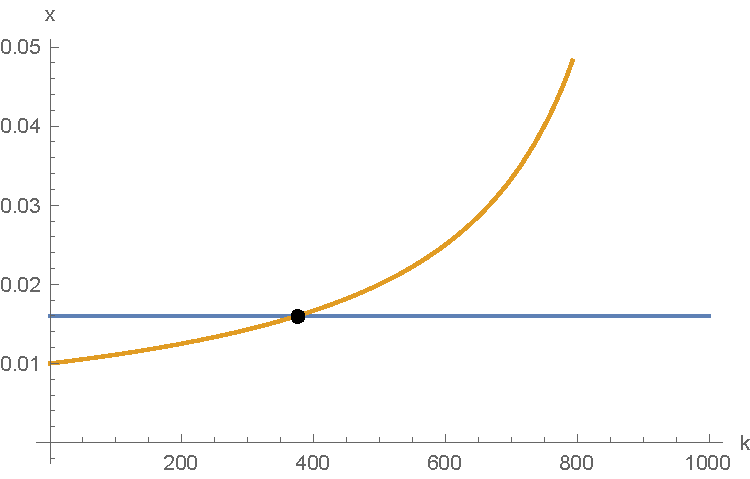
\includegraphics[width=0.45\textwidth]{Prob1_CapOpt/xopt_k.pdf}}
		\subfigure[Evaluation of value functions $F$, considering capacities $K=100$ (darker blue) and $K=700$ (lighter blue), and $F^*$ (orange) with respective demand threshold values presented (black)]{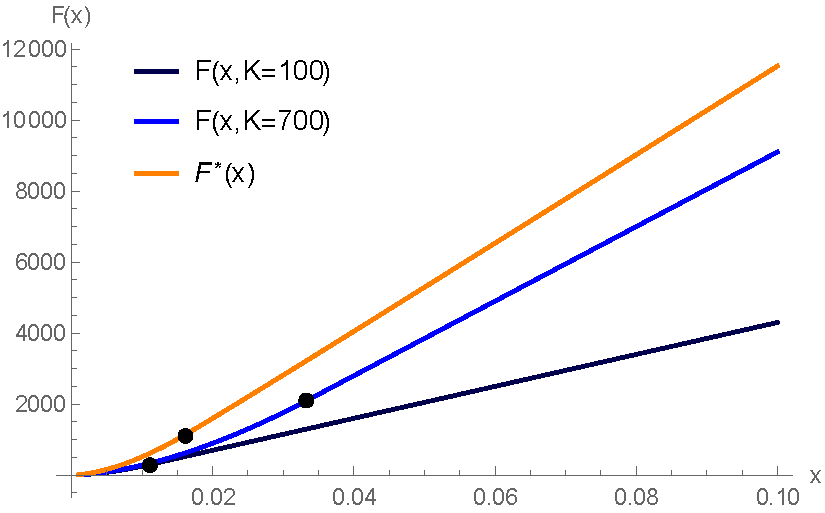
\includegraphics[width=0.45\textwidth]{Prob1_CapOpt/F_k100700.pdf}}
	\end{subfigmatrix}
	\caption{Influence of the chosen capacity $K$ in the threshold values $x^*_B$ and $x^*_C$ and respective value functions $F$ and $F^*$.}
	\label{fig:Kvar}
\end{figure}

We start by illustrating how $x^*_B$ and $x^*_C$ are related by the capacity level $K$, on which $x^*_B$ is dependent. The leftmost side of Figure \ref{fig:Kvar} comproves the results stated in Propositions \ref{1_prop1} and \ref{1_prop2} are valid: the threshold $x^*_B$ increases with capacity $K$.

Note that, although the threshold $x_B^*$ may be smaller or bigger (depending on the capacity $K$ chosen), we will always observe $F^*(x) \geq F(x,K) \ \forall x, K$ parameters considered in the domain of our problem, as can be seen on the rightmost side of Figure \ref{fig:Kvar}. Here we have represented value functions $F(x,K)$ defined as in \eqref{1_F}, with the dependence on the capacity $K$ highlighted, and $F^*$ is as defined in \eqref{1_F*}. 



\begin{figure}[!htb]
	\begin{subfigmatrix}{3}
		\subfigure[$r \in ( \mu, 1)$]{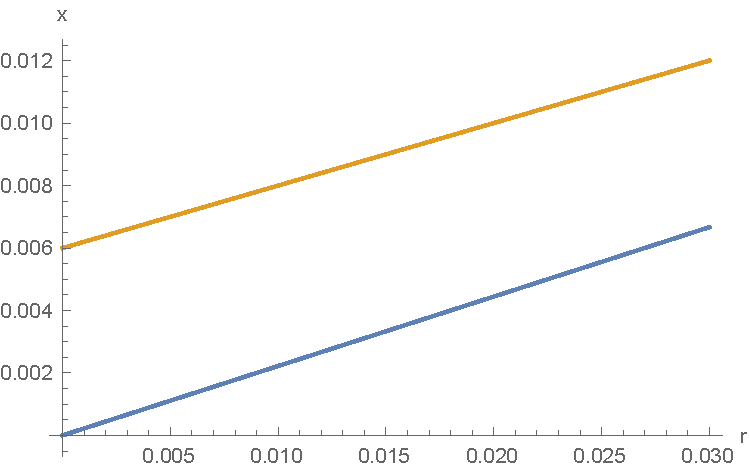
\includegraphics[width=0.32\textwidth]{Prob1_CapOpt/xopt_r.pdf}}
		\subfigure[$\sigma \in (0.0001,1)$]{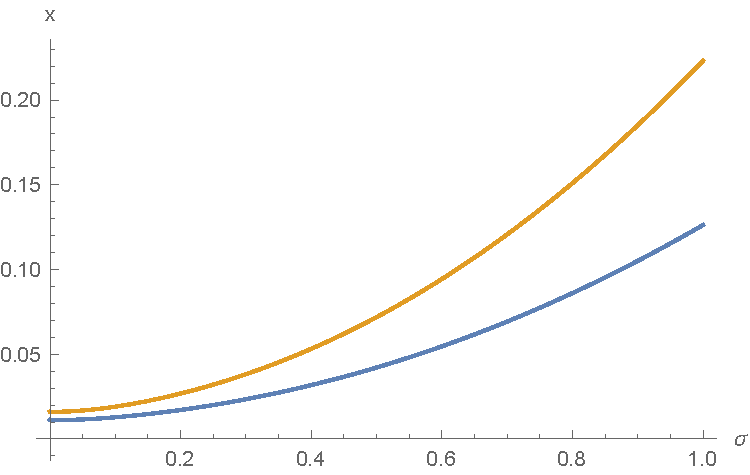
\includegraphics[width=0.32\textwidth]{Prob1_CapOpt/xopt_sigma.pdf}}
		\subfigure[$\delta \in (0,10)$]{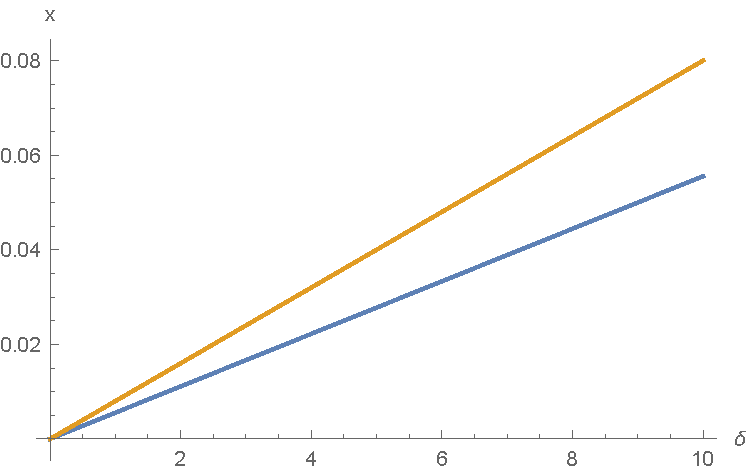
\includegraphics[width=0.32\textwidth]{Prob1_CapOpt/xopt_delta.pdf}}
	\end{subfigmatrix}
	\caption{Threshold value with respect to the benchmark model (blue) and the capacity optimized model (orange) and regarding its increasing parameters $r, \ \sigma$ and $\delta$.}
	\label{fig:sigm}
\end{figure}

On Figure \ref{fig:sigm} we observe that both thresholds increase with volatility. This in accordance with \cite{rita} and \cite{hagspiel:cap}, whose works describe that when uncertainty is high, there is a delay time to invest, which is here reflected on an higher demand level.

As the sensibility parameter $\delta$ increases, the firm needs to pay more sunk costs. Therefore the investment will only be made if higher demand values are observed, which is comproved also by Figure \ref{fig:sigm}.

On the other side, as the discount rate $r$ increases, we have a bigger currency devaluation, when evaluating the expected cash-flow to be earned. Thus, in order to justify the irreversible investment that the firm needs to incur on the new product, we need to observe bigger values of demand to balance the money lost due to currency devaluation and the future earnings.


\begin{figure}[!htb]
	\begin{subfigmatrix}{2}
		\subfigure[$\sigma=0.05$]{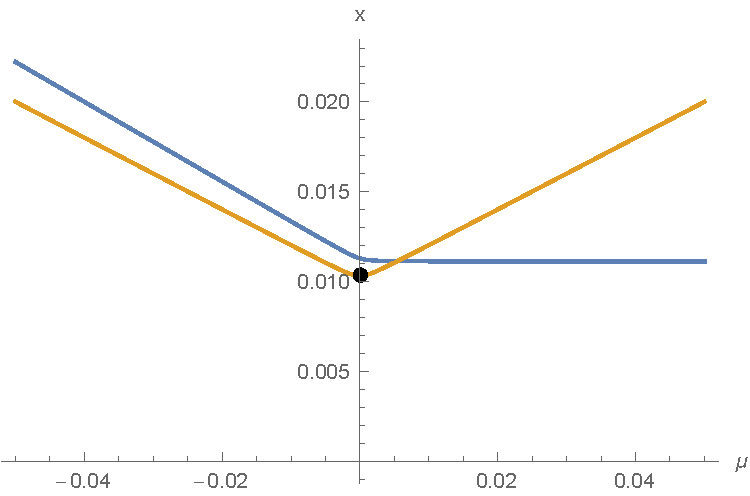
\includegraphics[width=0.45\textwidth]{Prob1_CapOpt/xopt_mu.pdf}}
		\subfigure[$\sigma=0.2$]{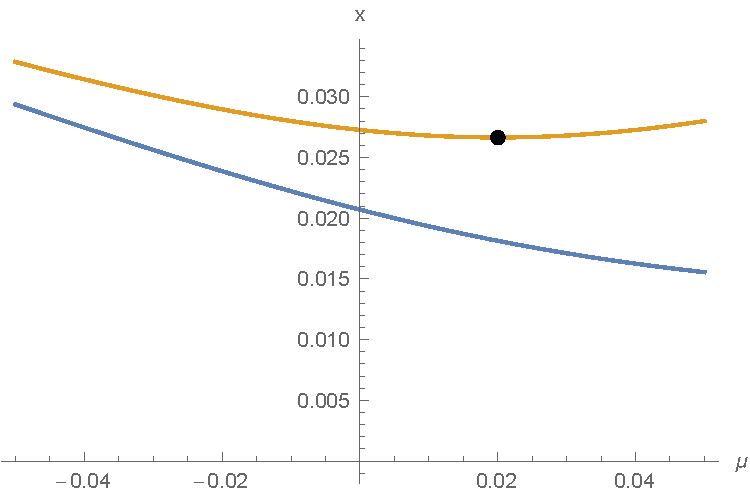
\includegraphics[width=0.45\textwidth]{Prob1_CapOpt/xopt_mu_sigma2.pdf}}
	\end{subfigmatrix}
	\caption{Threshold value with respect to the benchmark model (blue) and the capacity optimized model (orange), considering drift $\mu \in [-r, r]$ and corresponding stationary point $\sigma^2/2$ (black).}
	\label{fig:mu}
\end{figure}

Regarding the drift parameter $\mu$ we obtained that the threshold values do not have a monotonic behaviour, either for smaller or bigger values of volatility. As showed in Figure \ref{fig:mu}, the smallest value of demand level necessary to invest is observed at the stationary point when $\mu=\sigma^2/2$.



\begin{figure}[!htb]
	\centering
	\subfigure[$\theta \in ( 1, 10)$ ]{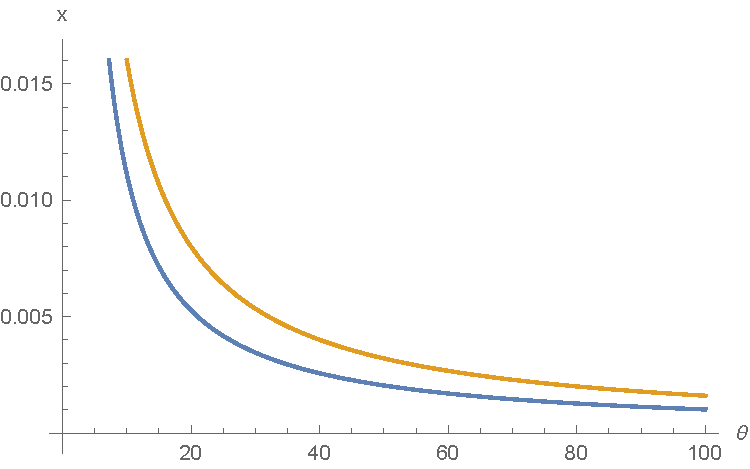
\includegraphics[width=0.45\textwidth]{Prob1_CapOpt/xopt_theta.pdf}}
	\caption{Threshold values regarding the benchmark model (blue) and the capacity optimized model (orange) and decreasing parameter $\theta$.}
	\label{fig:td}
\end{figure}


Regarding the innovation breakthrough we observe, on Figure \ref{fig:td}, that a higher $\theta$ implies a smaller demand threshold, regarding both models. This is in accordance to what was done in \cite{rita}, since as $\theta$ increases, the firm wills to invest in a product with much more advanced technology, that, taking into account our instantaneous profit function $\pi$ \eqref{prob1:pi}, will culminate in higher earnings, when fixing the demand value.



\subsection{Optimal Capacity Level}

Now that the threshold values were analysed, we focus on the optimal capacity $K^*_C$ as it is presented in \eqref{prob1:K*}. We analyse how does $K_C^*$ behaves with the different parameters.

\begin{prop}
	\label{1_prop3}
Optimal capacity level $K^*_C$ increases with $\mu$, $\sigma$ and $\theta$, decreases with $r$ and $\alpha$ and it is not dependent on $\delta$.
\end{prop}


\textbf{Proof:}
The relation between $K^*_C$ and $\theta$, $r$ or $\alpha$ comes immediately by observing $K^*_C$ expression.

Now, regarding drift parameter we obtain that
 \begin{align*}
\frac{\partial K^*_C(\mu)}{\partial \mu}=
\frac{4 \theta \left(\sigma ^2 \left(\phi+1\right)-2 \mu \right)}{\alpha \phi \left(\sigma ^2 \left(\phi+3\right)-2 \mu \right)^2}>0.
\end{align*}
Since
\begin{align}
\label{cond2}
\sigma ^2 \left(\sqrt{\frac{4 \mu ^2}{\sigma ^4}-\frac{4 \mu }{\sigma ^2}+\frac{8 r}{\sigma ^2}+1}+1\right)-2 \mu>0 
& \Leftrightarrow
\frac{4 \mu ^2}{\sigma ^4}-\frac{4 \mu }{\sigma ^2}+\frac{8 r}{\sigma ^2}+1 > \left( \frac{2 \mu}{\sigma^4}-1 \right)^2=\frac{4 \mu ^2}{\sigma ^4}-\frac{4 \mu }{\sigma ^2}+1 \\
& \Leftrightarrow
\frac{8 r}{\sigma ^2}>0, \nonumber
\end{align}
which is true for $\forall r> 0$. Therefore, it follows that the numerator is positive. Since $\phi>0$ \ref{phi}, it follows that the numerator is positive. From these two conditions, the result follows.

Regarding volatility parameter we obtain that
\begin{equation*}
    \frac{\partial K^*_C(\sigma)}{\partial \sigma}= 
\frac{8 \theta \left(2 \mu ^2-\mu  \sigma ^2 \left( \phi+1 \right)+2 r \sigma ^2 \right)}{\alpha \sigma  \phi  \left( \sigma ^2 \left( \phi+3 \right)-2 \mu \right)^2}>0
\end{equation*}

One can easily note that the denominator is positive.
When it comes to the numerator, we will study the sign of the expression between parenthesis.
\begin{align}
2 \mu ^2-\mu  \sigma ^2 \left(\phi+1\right)+2 r \sigma ^2 >0 & \Leftrightarrow \left( \frac{2 \mu^2+2r \sigma^2}{\mu \sigma^2} -1 \right)^2 > \frac{4 \mu^2}{\sigma^2}-\frac{4 \mu}{\sigma^2}+\frac{8r}{\sigma^2}+1\\
& \Leftrightarrow r>\mu,
\end{align}
which always hold, implying that the denominator is always positive.

%From \eqref{demo} we obtain that the denominator is positive and from \eqref{condd1} and \eqref{cond2} that the denominator is positive for $\forall r\geq0$, from which the result holds.
\begin{flushright}
	$\square$
\end{flushright}



\begin{figure}[!htb]
	\begin{subfigmatrix}{3}
		\subfigure[$\mu \in ( -r,r )$ ]{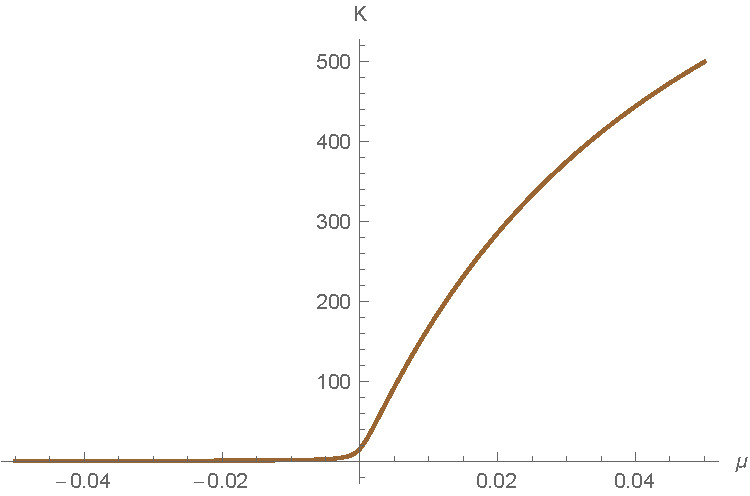
\includegraphics[width=0.32\textwidth]{Prob1_CapOpt/kopt_mu.pdf}}
		\subfigure[$\sigma \in (0,1)$]{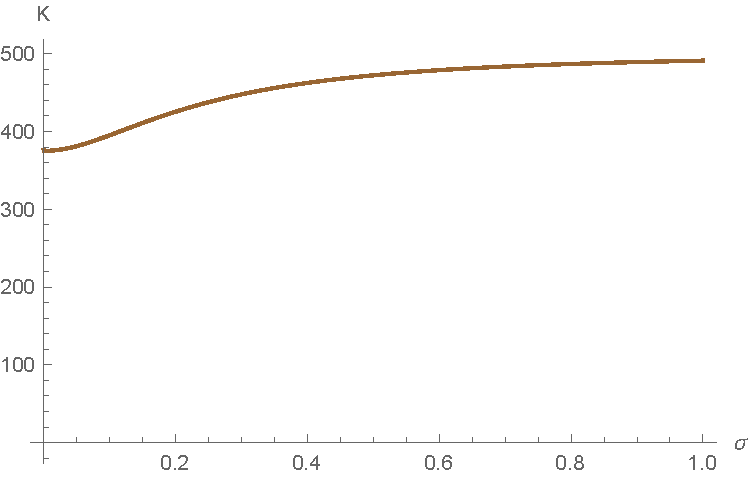
\includegraphics[width=0.32\textwidth]{Prob1_CapOpt/kopt_sigma.pdf}}
		\subfigure[$\theta \in (\alpha K^*_C,10)$]{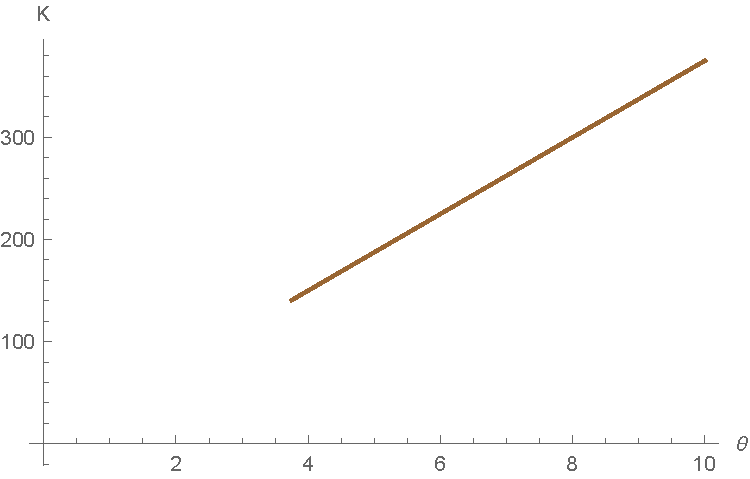
\includegraphics[width=0.32\textwidth]{Prob1_CapOpt/kopt_theta.pdf}}
	\end{subfigmatrix}
	\caption{Optimal capacity regarding the threshold value $x^*_C$ and increasing parameters $\mu$, $\sigma$ and $\theta$.}
	\label{fig:k1}
\end{figure}

Considering some numerical approximations, we observe, on Figure \ref{fig:k1}, that $K^*_C$ increases with drift, volatility and innovation level, as deduced before. Note that, regarding the drift parameter, the growth is barely noticeable for negative values of $\mu$, but then it turns to be logarithmic.
This is related with the fact that the denominator of $K_C^*$ decreases with $\mu$. For $\mu<0$, the denominator increases in a weak rate, resulting in an almost constant value of $K^*_C$. However, when $\mu>0$, as it increases, the denominator decreases significantly, resulting in higher values of $K^*_C$.

Regarding volatility $\sigma$, we obtain that the optimal capacity increases with it, however in a weaker rate.

Regarding the innovation breakthrough $\theta$, $K^*_C$ shows to increase linearly with it.
%FINANCIAL INTERPRETATION? This seems to be related with the fact that for small drift values, the future expected demand value is smaller that for positive drift values. Recall that the demand process evolves accordingly to a GBM and its expected value at time $t$ is given by $\mathds{E} ^{X_0=x_0} [X_t]=x_0 e^{\mu t}$.

\begin{figure}[!htb]
	\begin{subfigmatrix}{2}
		\subfigure[$ r \in ( \mu, 1 )$]{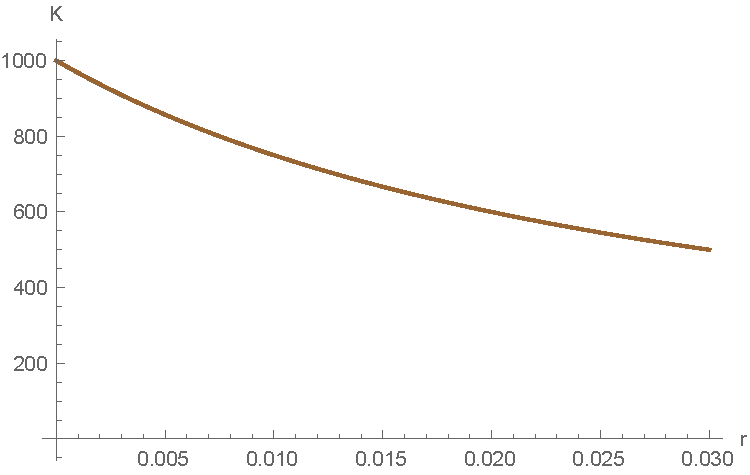
\includegraphics[width=0.45\textwidth]{Prob1_CapOpt/kopt_r.pdf}}
		\subfigure[$ \alpha \in (0,1)$]{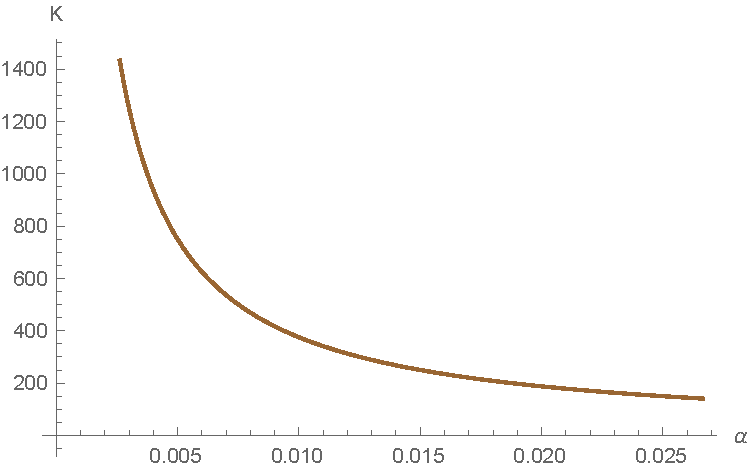
\includegraphics[width=0.45\textwidth]{Prob1_CapOpt/kopt_alpha.pdf}}
	\end{subfigmatrix}
	\caption{Optimal capacity regarding the threshold value $x^*_C$ and decreasing parameters $r$ and $\alpha$.}
	\label{fig:k2}
\end{figure}

Regarding discount rate $r$ and sensibility parameter $\alpha$, we have on Figure \ref{fig:k2} that $K^*_C$ decreases with them, as presented before in Proposition \ref{1_prop3}.
 
